\section{Theoretical basis of AI}
\subsection{AI algorithms for classification}
From a theoretical point of view many AI algorithms are formulated in terms of classification, i.e. a pattern recognition problem can be formulated as a classification problem. 
\\\\
A data set consists from cases (objects) and each case is characterised by some features, each case can be represented by a vector of features such that $\overrightarrow{x} = (x_1,x_2,...,x_p)$  each vector can be considered as a dot in p-dimensional space and all cases together form a cloud. If we Assume that each vector belongs to some class, the number of classes is M. The goal is to find a classifier that assigns to each case a label of some class.
\subsubsection{What a computer can see}
An image classifier takes a single image and assigns probabilities to labels. For an image of size $248\times400$ pixels and three colour channels, the image will consist of 297,600 numbers where each number is an an integer in a range from 0 to 255, our task if turn these numbers into a label.
\subsection{Data pre-processing}
There are four common forms of data pre-processing: centering, normalisation, dimensionality reduction, noise cancelling. To understand these procedure we assume that our data has a random nature and we use probability theory and statistics to deal with random variable and data analysis. 
\\\\
A Data matrix $X$, where we will assume that $X$ is of size $[n,p]$ (where $n$ is the number of data ( cases), $p$ is the dimensionality of the feature vector).

\subsection{Normal distribution}
A continuous random variable $X$ which is bell-shaped and has mean (expectation) $\mu$ and standard deviation $\sigma$ is said to follow a Normal Distribution with
parameters $\mu$ and $\sigma$.
\\\\
In shorthand, $X \sim \mathcal{N}(\mu,\,\sigma^{2})\,.$
This may be given in \emph{standardised} form by using the transformation
\begin{equation}
    z = \frac{z - \mu}{\sigma} \rightarrow x = \sigma z+ \mu \text{, where } Z \sim \mathcal{N}(0,\,1)\,.
\end{equation}
The normal distribution is important because of the Central Limit Theorem which states that a sum of arbitrary random variables will have a distribution that is approximately normal. 
\subsection{Bivariate normal distribution }
The multivariate normal distribution is a generalisation of the univariate normal to two or more variables, Each element of a normally distributed random vector has a univariate normal distribution. In the simplest case there is no correlation among variables, and elements of the vectors are independent univariate normal random variables. 

\begin{figure}[htbp]
    \def\centerx{2}
    \def\centery{-1}
    
    \centering
    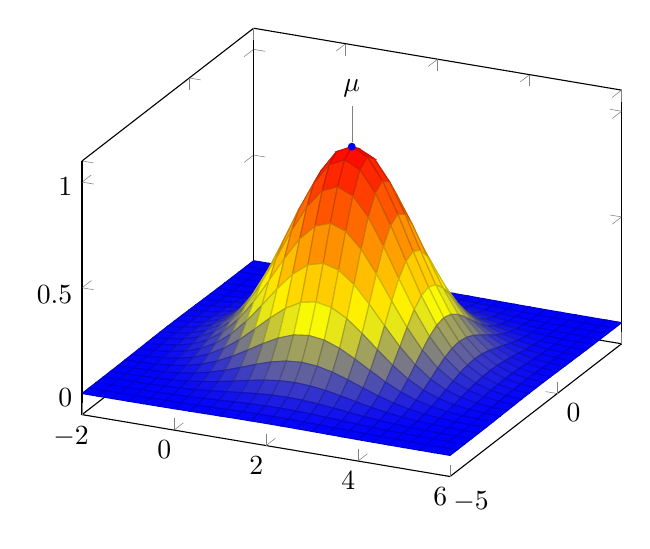
\begin{tikzpicture}
        \begin{axis}
        \addplot3[surf,domain=-2:6,domain y=-5:3] 
            {exp(-( (x-\centerx)^2 + (y-\centery)^2)/3 )};
        \node[circle,inner sep=1pt,fill=blue,pin=90:$\mu$] 
            at (axis cs:\centerx,\centery,1) {};
        \end{axis}
    \end{tikzpicture}
    \caption{Bivariate normal distribution 3D perceptive}
    \label{fig:my_label}
\end{figure}
\begin{figure}[htbp]
    \def\centerx{2}
    \def\centery{-1}
    \centering
    \begin{tikzpicture}
        \begin{axis}[view={0}{90},axis equal]
        \addplot3[contour gnuplot,domain=-2:6,domain y=-5:3] 
            {exp(-( (x-\centerx)^2 + (y-\centery)^2)/3 )};
        \node[circle,inner sep=1pt,fill=blue,pin=90:$\mu$] 
            at (axis cs:\centerx,\centery,1) {};
        \end{axis}
    \end{tikzpicture}
    \caption{Bivariate normal distribution 2D perceptive}
    \label{fig:my_label}
\end{figure}
$p$ is the correlation $-1 \leq p \leq 1$ 
\begin{itemize}
    \item $p = 0$ means that the varables are independent
    \item $p = +1$ means that the variables are linearly dependent
    \item $p = -1$ means also the linear dependence but the increase of one variable is associated with the decrease of an other.
\end{itemize}
\subsection{Statistics: Random sample}
Statistics is an interface between the probability theory and data, it provides multiple procedures for data analysis. In statistics the data set is a sample, this sample should be chosen in a proper way and correctly represent a random variable which we would like to estimate.
\subsection{Parameter estimators}
Data analysis is based of statistical estimator of the random variable $X$, i.e. for sample $X = (x_1,x_2,...,x_n)$, 
\\\\
The estimator of the mean is
\begin{equation}
  \Bar{X} = \frac{1}{n}\sum_{i=1}^{n} x_i.
\end{equation}
The estimator of the variance is 
\begin{equation}
  S_x^2 = \frac{1}{n} {\sum_{i=1}^{n} (x_i - \Bar{X})^2}.
\end{equation}
The estimator of the standard deviation is 
\begin{equation}
    S_x = \sqrt{\frac{1}{n} {\sum_{i=1}^{n} (x_i - \Bar{X})^2}}
\end{equation}
Now consider the bivariate random variable $(X,Y) = \{(x_i,y_i)\},i = 1,2,...,n$
\\\\
The estimator of the covariance is 
\begin{equation}
    cov(X,Y) = \frac{1}{n-1} {\sum_{i=1}^{n} (x_i - \Bar{X})}(y_i - \Bar{Y})}
\end{equation}
The estimator of the correlation is 
\begin{equation}
    p = \frac{cov(X,Y)}{S_x S_y}
\end{equation}
\subsection{Data Centering}
Mean subtraction is the most common form of pre-processing, it involves subtracting $\mu$ across every individual feature in the data and has the geometric interpretation of centering the cloud of data around the origin along every dimension. 
\subsection{Data normalisation}
Normalisation referees to normalising the data dimensions so that they are approximately the same scale. There are two common ways of achieving this normalisation
\begin{enumerate}
    \item To divide each dimension by its standard deviation, once it has been zero centered
    \item normalised each dimension so that the min and max along the dimension is -1 and 1 respectively
\end{enumerate}
It only makes sense to apply this pre-processing if you have a reason to believe that different input features have different scales, but thy should be approximately equal importance to the learning algorithm. In the cases of images the relative scales of pixels are already approximately equal, so it is not strictly necessary to perform this addition pre-processing step.
\subsection{Dimensionality reduction: Principal Component Analysis (PCA)} 
Principal components analysis is a quantitatively rigorous method for achieving data simplification and dimensionality reduction. The method generates a new set of variables, called principal components.  Each principal component is a linear combination of the original variables. All the principal components are orthogonal to each other, so there is no redundant information. The principal components as a whole form an orthogonal basis for the space of the data.
\begin{enumerate}
    \item The first principal component is a single axis in space. When you project each observation on that axis, the resulting values form a new variable. The variance of this variable is the maximum among all possible choices of the first axis. 
    \item The second principal component is another axis in space, perpendicular to the first. Projecting the observations on this axis generates another new variable. The variance of this variable is the maximum among all possible choices of this second axis.
    \item The full set of principal components is as large as the original set of variables. But it is a common place for the sum of the variances of the first few principal components to exceed 80\% of the total variance of the original data. 
\end{enumerate}
\subsection{Classify images}
The problem is very simple for natural intelligence, but very challenging for the AI. Recent Google developments of Convolutional Neural Networks (CNN) allow to the solve this problem and classify images with a small amount of error
\subsection{Binary (two classes) classification}
If we simplify the image problem down to dots on a 2-dimensional plane and would like to classify them, the idea would be to find the separator between the two classes the simplest separator is a straight line. 
\subsection{Linear Regression}
Regression is the task of predicting real valued quantities. For this type of task, it is common to compute the error function between the predicted quantity and  the true answer, the error function includes both data and parameters. Minimization of the error function provides optimal parameter values.
\subsubsection{Least squares}
Linear regression line is the line of best fit: the sum of squared distances from the data point to the line is the smallest ( least squares).
\\\\
This is niavie and simple approach however it shows a typical approach to the construction of an AI algorithm.
\begin{itemize}
    \item Define an error function, which includes data and parameters
    \item Find min/max of this function according to the parameter variation (a training data set is given and fixed)
    \item Optimization procedure provides the optimal parameter values which define the best classifier for the given training set.
\end{itemize}
The solution of this optimization problem (i.e. the parameter values corresponding to the global minimum or some point nearby) is the best set of parameter values for the classifier
\subsection{Numerical optimization}
There two main numerical methods to solve the optimization problem 
\subsubsection{Gradient descent}
The vector gradient is defined as
\begin{equation}
    \nabla f = \Big(\frac{\delta f}{\delta x}, \frac{\delta f}{\delta y} \Big)^T
\end{equation}
Gradient descent uses just the gradient of the function to navigate to the minimum. From
calculus, the direction of − $\nabla$ f is that of maximum change of the function. The gradient descent uses - $\nabla$ f (the down-gradient direction) as an estimate of the direction of the minimum
\subsubsubsection{Multivariable calculus: gradient}
The gradient is a vector having direction equal to the greatest rate of increase, and magnitude equal to the slope of the function in that direction.
\begin{itemize}
    \item  The Jacobian Matrix is defined for scalar-valued functions (functions with a single output), whereas for vector-valued functions it is necessary to use the Jacobian matrix.
\end{itemize}
\subsubsection{Higher dimensional Newton-Raphson}
In cases where the first derivative $f'(x)$ is well behaved in the region of the root, we can used the Newton-Raphson method to compute the root. 
\begin{equation}
    X_{n+1} = X_n - J^{-1}(X_n)F(X_n)
\end{equation}
\subsubsubsection{Example}
Consider finding the roots of the two functions
$$
    f(x,y) = 9- x^4-y^4
$$
$$
    g(x,y) = x^2-2y+2
$$
Starting at
$$
    x_0 = \begin{pmatrix} 1 \\ 1 \end{pmatrix}
$$
The Jacobian is 
$$
    \begin{pmatrix} \frac{\delta f}{\delta x} & \frac{\delta f}{\delta y} \\ \frac{\delta g}{\delta x} & \frac{\delta g}{\delta y} \end{pmatrix} = \begin{pmatrix} -4x^3 & -4y^3 \\ 2x & -2 \end{pmatrix}
$$
The first step of the 2D Newton-Raphson method is:
\begin{equation*}
    X_{1} = X_0 - J^{-1}(X_0)F(X_0)
\end{equation*}
\begin{equation*}
   \begin{pmatrix} x_1 \\ y_1 \end{pmatrix} =  \begin{pmatrix} 1 \\ 1 \end{pmatrix} - \frac{1}{8} \begin{pmatrix} -1 & 2 \\ -1 & -2 \end{pmatrix}\begin{pmatrix} 7 \\ 1 \end{pmatrix} = \begin{pmatrix} 1.625 \\ 2.125 \end{pmatrix}
\end{equation*}
